

\tikzset{every picture/.style={line width=0.75pt}} %set default line width to 0.75pt        

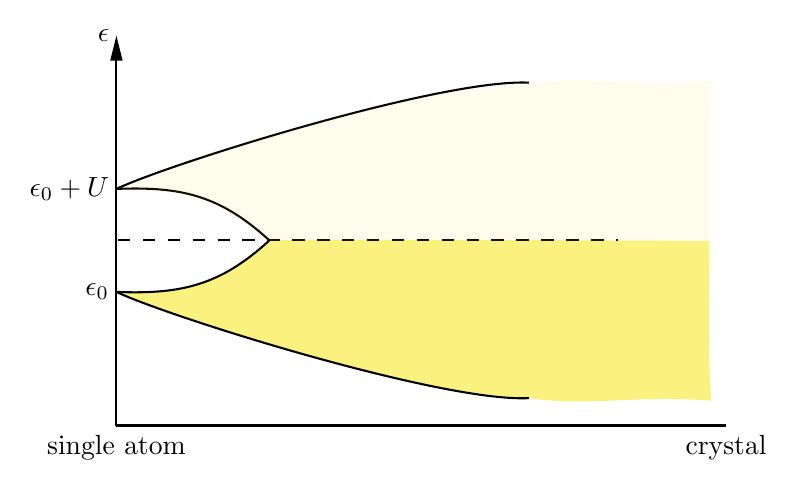
\begin{tikzpicture}[x=0.75pt,y=0.75pt,yscale=-1,xscale=1]
%uncomment if require: \path (0,300); %set diagram left start at 0, and has height of 300

%Shape: Polygon Curved [id:ds7075624570459664] 
\draw  [draw opacity=0][fill={rgb, 255:red, 248; green, 231; blue, 28 }  ,fill opacity=0.57 ] (173,213.63) .. controls (198.71,216.07) and (226.71,209.07) .. (246.71,188.81) .. controls (296.71,188.07) and (439.71,189.07) .. (458.71,189.07) .. controls (458.71,210.07) and (457.71,245.07) .. (459.71,266.07) .. controls (422.71,263.07) and (401.71,269.07) .. (371.71,264.81) .. controls (315.71,262.07) and (231.71,237.07) .. (173,213.63) -- cycle ;
%Straight Lines [id:da8100808760339464] 
\draw    (173,278) -- (466.71,278) ;
%Straight Lines [id:da1730446730702535] 
\draw    (173,92.19) -- (173,278) ;
\draw [shift={(173,90.19)}, rotate = 90] [fill={rgb, 255:red, 0; green, 0; blue, 0 }  ][line width=0.08]  [draw opacity=0] (12,-3) -- (0,0) -- (12,3) -- cycle    ;
%Curve Lines [id:da37288245167395306] 
\draw    (173,164) .. controls (203.71,162.81) and (222.71,166.81) .. (246.71,188.81) ;
%Curve Lines [id:da1329203045652183] 
\draw    (173,213.63) .. controls (203.71,214.81) and (222.71,210.81) .. (246.71,188.81) ;
%Curve Lines [id:da9577944633435271] 
\draw    (173,164) .. controls (198.71,151.81) and (329.71,110.81) .. (371.71,112.81) ;
%Curve Lines [id:da3428932734540302] 
\draw    (173,213.63) .. controls (198.71,225.81) and (329.71,266.81) .. (371.71,264.81) ;
%Straight Lines [id:da604449076641173] 
\draw  [dash pattern={on 4.5pt off 4.5pt}]  (173.71,188.81) -- (414.71,188.81) ;
%Shape: Polygon Curved [id:ds33698675422401303] 
\draw  [draw opacity=0][fill={rgb, 255:red, 248; green, 231; blue, 28 }  ,fill opacity=0.08 ] (173,164.52) .. controls (198.71,162.07) and (226.71,169.07) .. (246.71,189.33) .. controls (296.71,190.07) and (439.71,189.07) .. (458.71,189.07) .. controls (458.71,168.07) and (457.71,133.07) .. (459.71,112.07) .. controls (422.71,115.07) and (401.71,109.07) .. (371.71,113.33) .. controls (315.71,116.07) and (231.71,141.07) .. (173,164.52) -- cycle ;

% Text Node
\draw (173,281) node [anchor=north] [inner sep=0.75pt]   [align=left] {single atom};
% Text Node
\draw (466.71,281) node [anchor=north] [inner sep=0.75pt]   [align=left] {crystal};
% Text Node
\draw (171,90.19) node [anchor=east] [inner sep=0.75pt]    {$\epsilon $};
% Text Node
\draw (171,213.63) node [anchor=east] [inner sep=0.75pt]    {$\epsilon _{0}$};
% Text Node
\draw (171,164) node [anchor=east] [inner sep=0.75pt]    {$\epsilon _{0} +U$};


\end{tikzpicture}
